\section{Elementi di Matplotlib}

\subsection{Grafici a Dispersione}
Matplotlib è una libreria per la creazione di grafici in Python. Esempio di grafico a dispersione:
\begin{lstlisting}[language=Python]
import matplotlib.pyplot as plt
import numpy as np

x = np.random.rand(50)
y = np.random.rand(50)

plt.scatter(x, y)
plt.title("Grafico a Dispersione")
plt.xlabel("X")
plt.ylabel("Y")
plt.savefig('grafico_dispersione.png')
#se vuoi scaricare il file da google colab decommenta le righe:
#from google.colab import files
#files.download('grafico_dispersione.png')
plt.show()
\end{lstlisting}

Includi il grafico nel documento:
\begin{figure}[h!]
    \centering
    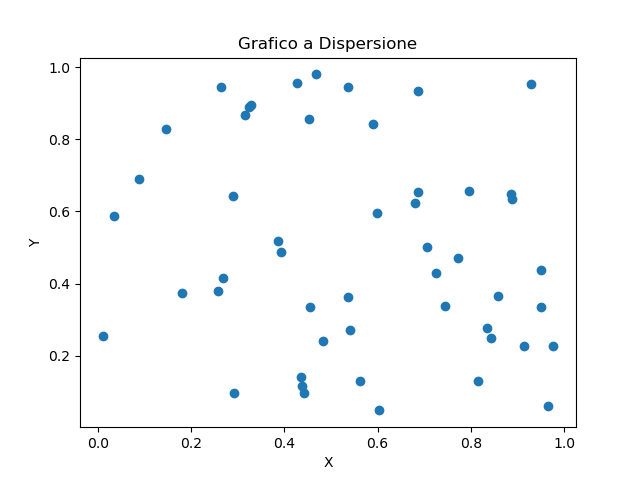
\includegraphics[width=0.8\textwidth]{grafico_dispersione.png}
    \caption{Grafico a Dispersione}
    \label{fig:grafico_dispersione}
\end{figure}

\subsection{Grafici con Barre di Errore}
I grafici con barre di errore mostrano l'incertezza nei dati. Esempio:
\begin{lstlisting}[language=Python]
import matplotlib.pyplot as plt
import numpy as np

x = np.linspace(0, 10, 10)
y = np.sin(x)
yerr = 0.2

plt.errorbar(x, y, yerr=yerr, fmt='-o')
plt.title("Grafico con Barre di Errore")
plt.xlabel("X")
plt.ylabel("Y")
plt.savefig('grafico_barre_errore.png')
#se vuoi scaricare il file da google colab decommenta le righe:
#from google.colab import files
#files.download('barre_errore.png')
plt.show()
\end{lstlisting}

Includi il grafico nel documento:
\begin{figure}[h!]
    \centering
    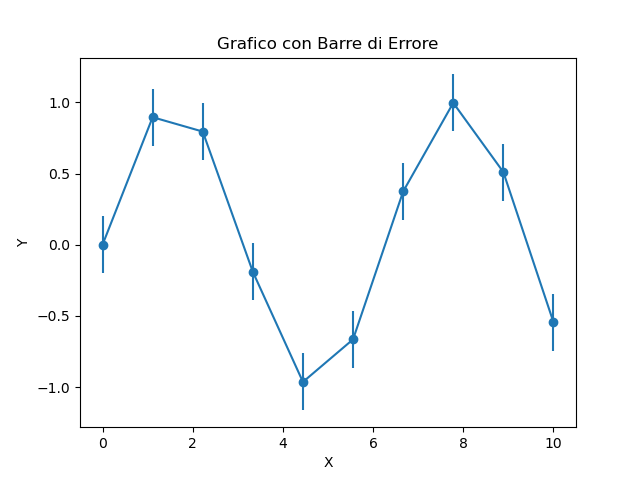
\includegraphics[width=0.8\textwidth]{grafico_barre_errore.png}
    \caption{Grafico con Barre di Errore}
    \label{fig:barre_errore}
\end{figure}

\subsection{Grafico Spazio-Tempo e Velocità-Tempo per Moto Uniforme a Tratti}
Consideriamo un moto uniforme a tratti, dove un oggetto si muove a tre diverse velocità in tre intervalli di tempo distinti. Creiamo due grafici: uno per il moto spaziale-temporale e uno per la velocità-tempo.

\subsubsection{Grafico Spazio-Tempo}
Nel grafico spazio-tempo, mostriamo il percorso dell'oggetto in funzione del tempo. Supponiamo che l'oggetto abbia velocità costanti di 2 m/s, 4 m/s e 6 m/s nei rispettivi intervalli di tempo.

Esempio di codice:
\begin{lstlisting}[language=Python]
import matplotlib.pyplot as plt
import numpy as np

# Dati
tempi = [0, 2, 5, 8, 10]
posizioni = [0, 4, 16, 28, 40]

# Creazione del grafico
plt.figure(figsize=(12, 6))
plt.plot(tempi, posizioni, marker='o')
plt.title("Grafico Spazio-Tempo per Moto Uniforme a Tratti")
plt.xlabel("Tempo (s)")
plt.ylabel("Posizione (m)")
plt.grid(True)
plt.savefig('grafico_spazio_temporale.png')
#se vuoi scaricare il file da google colab decommenta le righe:
#from google.colab import files
#files.download('grafico_spazio_temporale.png')
plt.show()
\end{lstlisting}

\subsubsection{Grafico Velocità-Tempo}
Il grafico velocità-tempo mostra la variazione della velocità in funzione del tempo. Ogni intervallo di tempo corrisponde a una velocità costante.

Esempio di codice:
\begin{lstlisting}[language=Python]
import matplotlib.pyplot as plt
import numpy as np

# Dati
tempi = [0, 2, 5, 8, 10]
velocita = [2, 2, 4, 4, 6]

# Creazione del grafico
plt.figure(figsize=(12, 6))
plt.step(tempi, velocita, where='post', marker='o')
plt.title("Grafico Velocità-Tempo per Moto Uniforme a Tratti")
plt.xlabel("Tempo (s)")
plt.ylabel("Velocità (m/s)")
plt.grid(True)
plt.savefig('grafico_velocita_temporale.png')
#se vuoi scaricare il file da google colab decommenta le righe:
#from google.colab import files
#files.download('grafico_velocita_temporale.png')
plt.show()
\end{lstlisting}

\subsubsection{Spiegazione dei Grafici}
\begin{itemize}
    \item \textbf{Grafico Spazio-Tempo:} Questo grafico mostra come la posizione dell'oggetto cambia nel tempo. È possibile osservare che il grafico è composto da segmenti lineari, ognuno con una pendenza diversa, che rappresenta le diverse velocità. L'area sotto la curva corrisponde alla distanza percorsa.
    \item \textbf{Grafico Velocità-Tempo:} Questo grafico mostra come la velocità cambia nel tempo. Utilizzando un grafico a passo, ogni intervallo di tempo mostra una velocità costante. Il grafico indica chiaramente le transizioni tra le diverse velocità.
\end{itemize}

Includi i grafici nel documento:
\begin{figure}[h!]
    \centering
    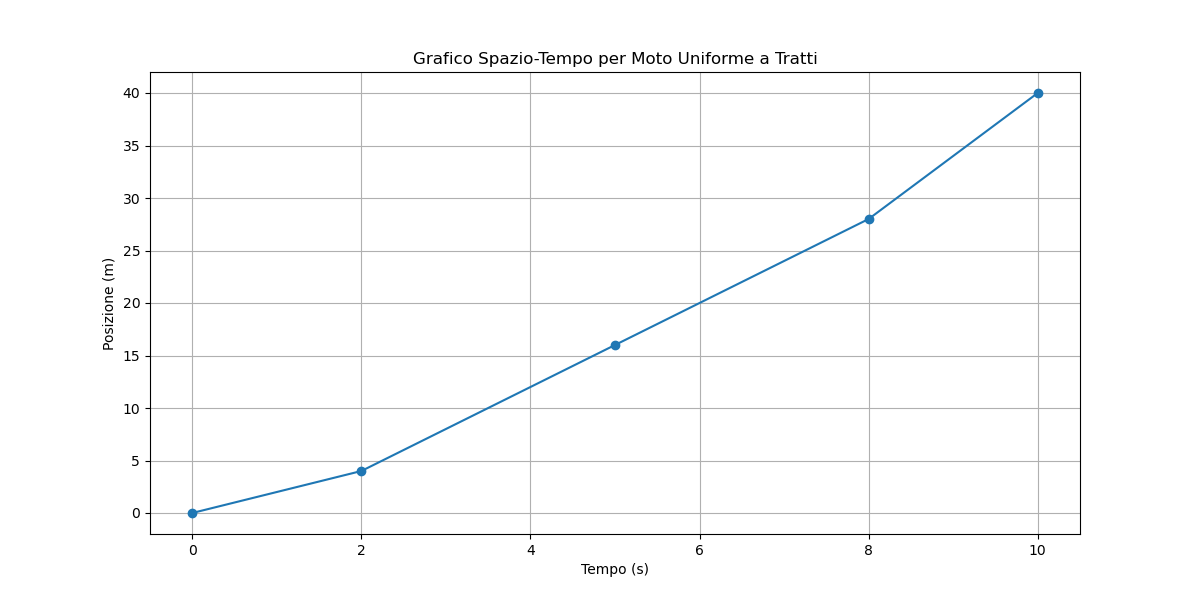
\includegraphics[width=0.8\textwidth]{grafico_spazio_temporale.png}
    \caption{Grafico Spazio-Tempo per Moto Uniforme a Tratti}
    \label{fig:spazio_temporale}
\end{figure}

\begin{figure}[h!]
    \centering
    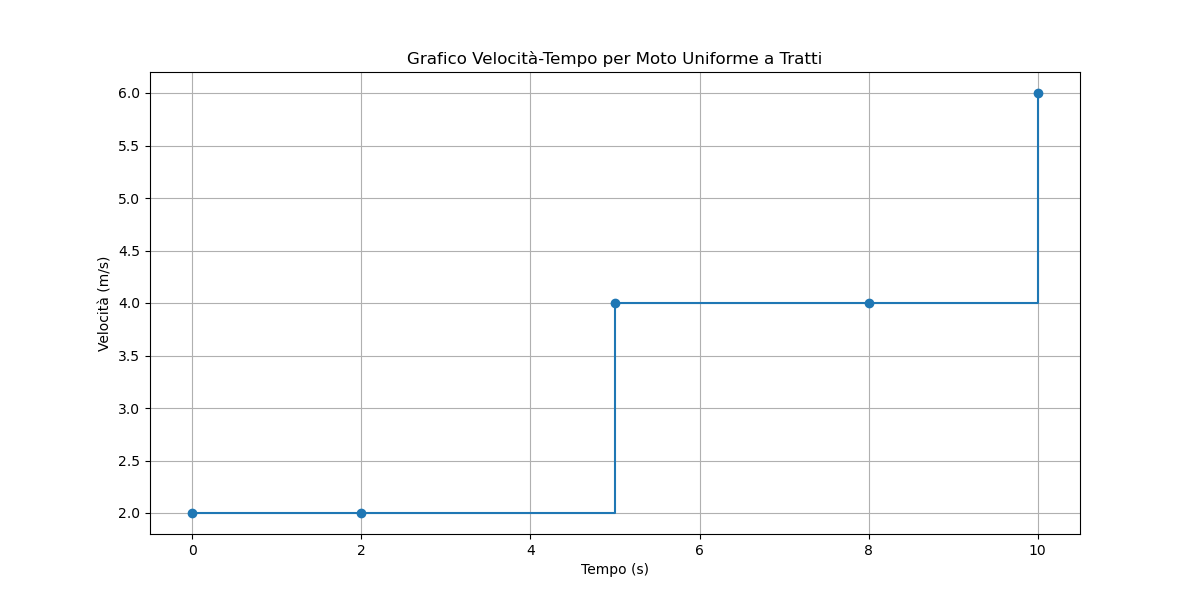
\includegraphics[width=0.8\textwidth]{grafico_velocita_temporale.png}
    \caption{Grafico Velocità-Tempo per Moto Uniforme a Tratti}
    \label{fig:velocita_temporale}
\end{figure}

\subsection{Grafico Altezza-Diametro di un Cilindro con Volume Fisso}
Infine, consideriamo un grafico che mostra come l'altezza di un cilindro varia in funzione del diametro della base, mantenendo fisso il volume.

Esempio di codice:
\begin{lstlisting}[language=Python]
import matplotlib.pyplot as plt
import numpy as np

# Costanti
volume = 1000  # Volume costante del cilindro in m³

# Diametro della base
diametro = np.linspace(1, 10, 100)  # Diametro varia da 1 a 10 metri

# Calcolo dell'altezza
altezza = volume / (np.pi * (diametro / 2)**2)

# Creazione del grafico
plt.figure(figsize=(12, 6))
plt.plot(diametro, altezza, label='Altezza = Volume / (pigreco x (Diametro / 2)^2)', color='green')
plt.title("Grafico dell'Altezza in Funzione del Diametro di Base (Volume Fisso)")
plt.xlabel("Diametro della Base (m)")
plt.ylabel("Altezza (m)")
plt.grid(True)
plt.legend()
plt.savefig('grafico_altezza_diametro.png')
#se vuoi scaricare il file da google colab decommenta le righe:
#from google.colab import files
#files.download('grafico_altezza_diametro.png')
plt.show()
\end{lstlisting}

Includi il grafico nel documento:
\begin{figure}[h!]
    \centering
    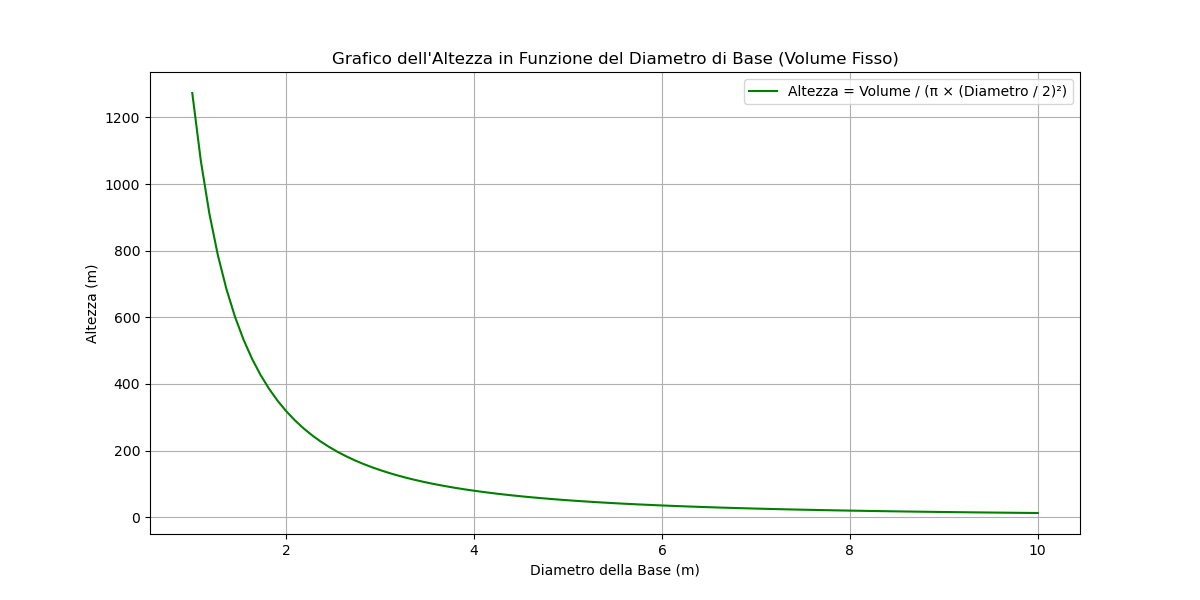
\includegraphics[width=0.8\textwidth]{grafico_altezza_diametro.png}
    \caption{Grafico dell'Altezza in Funzione del Diametro di Base (Volume Fisso)}
    \label{fig:altezza_diametro}
\end{figure}
\chapter{Statistica}
